\section{Evaluation}
\label{sec:eval}

We built two systems, one streams real-time TV videos and the other 
simulates the TV watching using the same weekly schedule. The latter, 
which is called ''PredicTV (survey)'', is necessary because capturing 
user behavior on real TV takes a lot of time, and a simulator significantly 
speeds up our evaluation. A total of 81 channels are included in the systems.

\subsection{Extraction}
The target of the extraction is to fill values in as many attributes as 
possible of the programs. The sufficiency and precision of the attribute-value 
pairs extracted are a big concern of the performance of our algorithm. We calculated the coverage of the values
on both the attributes (Figure \ref{fig:extraction}) and the programs, and also 
sampled 50 programs to verify the precision of the attribute values
(Table \ref{tab:extraction}).

By the statistics in the graph and table, the extraction result has plenty 
of information that can well support our algorithm.

\begin{figure}[h]
\begin{center}
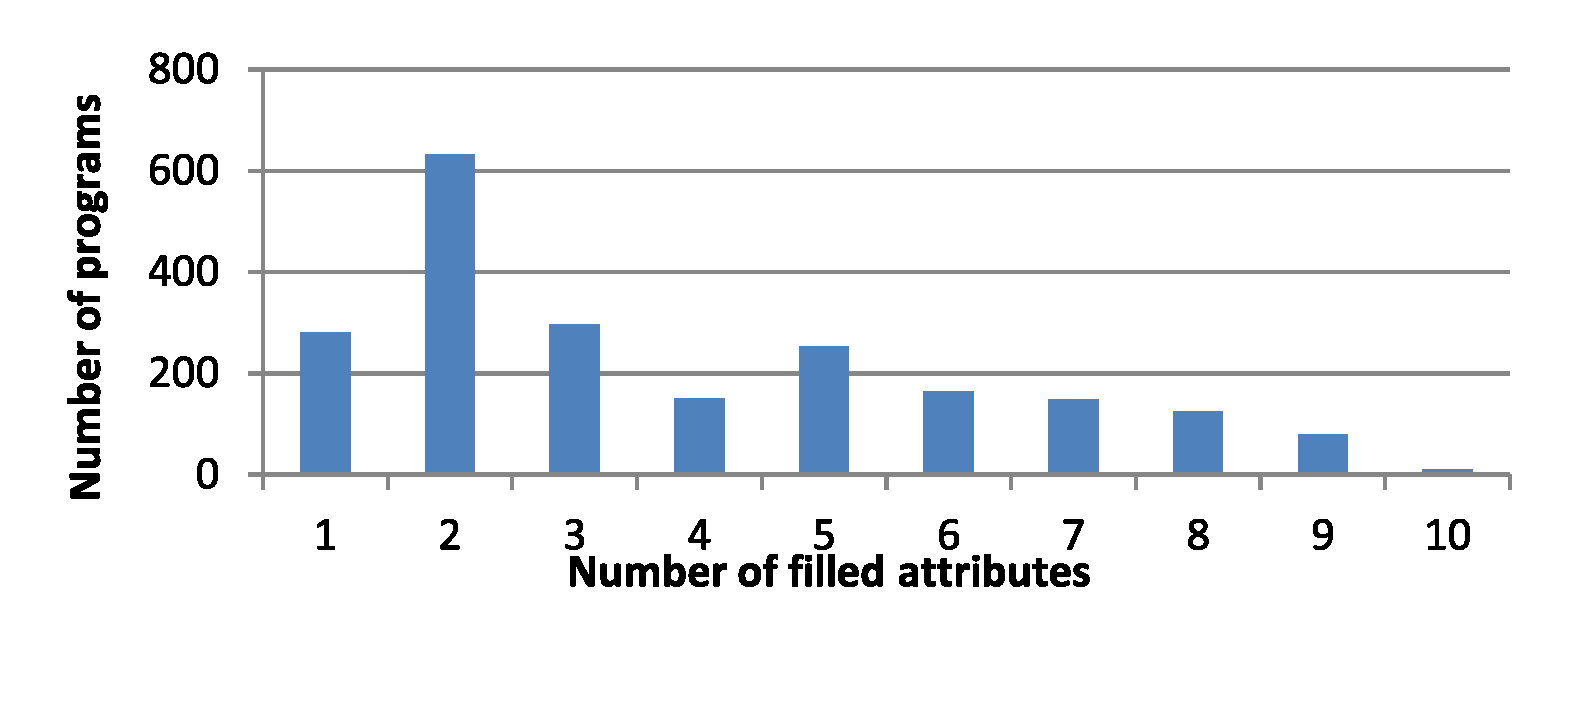
\epsfig{file=extract.eps,width=\columnwidth}
\caption{\label{fig:extraction}Programs distribution on number of attributes with values}
\end{center}
\end{figure}

\begin{table}[h]
\begin{center}
\begin{tabular}{|c|c|c|c|c|c|}
\hline
Attribute & Values & Programs & Sam. & Cor. & Prec. \\
\hline
\hline
Prog Name& 2137 & 2137 & 50 & 50 & 1.000 \\
\hline
Director & 774  & 486  & 23 & 17 & 0.717 \\
\hline
Producer & 385  & 157  & 28 & 21 & 0.750 \\
\hline
Region   & 1674 & 858  & 47 & 41 & 0.872 \\
\hline
Type     & 2647 & 975  & 85 & 56 & 0.659 \\
\hline
Language & 552  & 415  & 28 & 23 & 0.821 \\
\hline
Writer   & 506  & 306  & 29 & 20 & 0.690 \\
\hline
Actor    & 1760 & 537  & 59 & 48 & 0.814 \\
\hline
Host     & 975  & 566  & 34 & 25 & 0.735 \\
\hline
Category & 5799 & 1685 & 121& 83 & 0.686 \\
\hline
\bf{Overall}&17538 & 2137 & 527& 400& 0.759 \\
\hline
\end{tabular}
\end{center}
\tab Values = total \# of values on the attribute\\
\tab Programs = \# of programs with at least one value on the attribute\\
\tab Sam. = \# of data samples, Cor. = \# of correct samples\\
\tab Prec = estimated precision 
\caption{\label{tab:extraction}Program coverage and precision of the attributes}
\end{table}


\subsection{Recommendation}
20 users in 4 groups are invited to the experiment, in which they are asked 
to simulate watching TV in the first week of Apr. 2012 using the 
''PredicTV (survey)''. The 4 groups are 
given different recommendation algorithms for comparison purposes, none, 
random, collaborative filtering, and ours respectively, where collaborative 
filtering recommends a user the programs watched by others who share similar 
watching history with him.

We use coverage and predictability to measure the recommendations. Coverage 
is the percentage of the programs followed by the user among all that
recommended, or the ratio of the programs recommended over all that 
watched by the user (Table \ref{tab:coverage}).

\begin{table}[!hbp]
\begin{center}
\begin{tabular}{|c|c|c|c|c|}
\hline
                       & None &  Ran.  & CF  & PredicTV\\
\hline
\hline
Avg User Watched       & 71.8 &  60.8  & 68.6& \bf{83.2}\\
\hline
Avg Recommended        &  -   &  174.2 &158.0& \bf{203.6} \\
\hline
Avg Overlap            &  -   &  2.2   & 7.8 & \bf{27.2}  \\
\hline
Avg Recommend Followed &  -   &  0.013 &0.049& \bf{0.134} \\
\hline
Avg Watching Expected  &  -   &  0.036 &0.114& \bf{0.327} \\
\hline
\end{tabular}
\end{center}
Recommend Followed = \% of recommended programs actually watched by user\\
Watching Expected = \% of user watched programs covered by recommendation
\caption{\label{tab:coverage}User watching and recommendation coverage}
\end{table}

Predictability calculates the difference between the recommended programs and
the programs the user actually watches using a difference function. 
For example, having the recommendation 
list of Wednesday based on the watching history of Monday and Tuesday, we 
compare it with the program list the user actually watched on Wednesday.
We calculate the predictability as follows.
\begin{eqnarray*}
\rm{predictability} &=& \frac{1}{\sum_{a \in A} \rm{distance}(a,B)}\\
\rm{distance}(a, b) &=& \left\{
		\begin{array}{ll}
			| index_A(a)  - index_B(a)|    \tab(a \in B) \\
			| index_A(a) - len(B) |   \tab	(a \not\in B))
		\end{array}\right.
\end{eqnarray*}

In this way, we get the predictability of 7 days, and plot the variation
curve of the 3 algorithms based on the average predictability of 15 users
 (Figure \ref{fig:predict}). As is shown in the graph and the table, PredicTV is improving as more watching behaviors are captured, and it outperforms random
recommendation and collaborative filtering. The reason that CF performs 
so weak may be resulted from the cold start
\cite{Schein02:ColdStart}problem, as we only have 15 users' less than 1 week 
watching history to build the model.

\begin{figure}[h]
\begin{center}
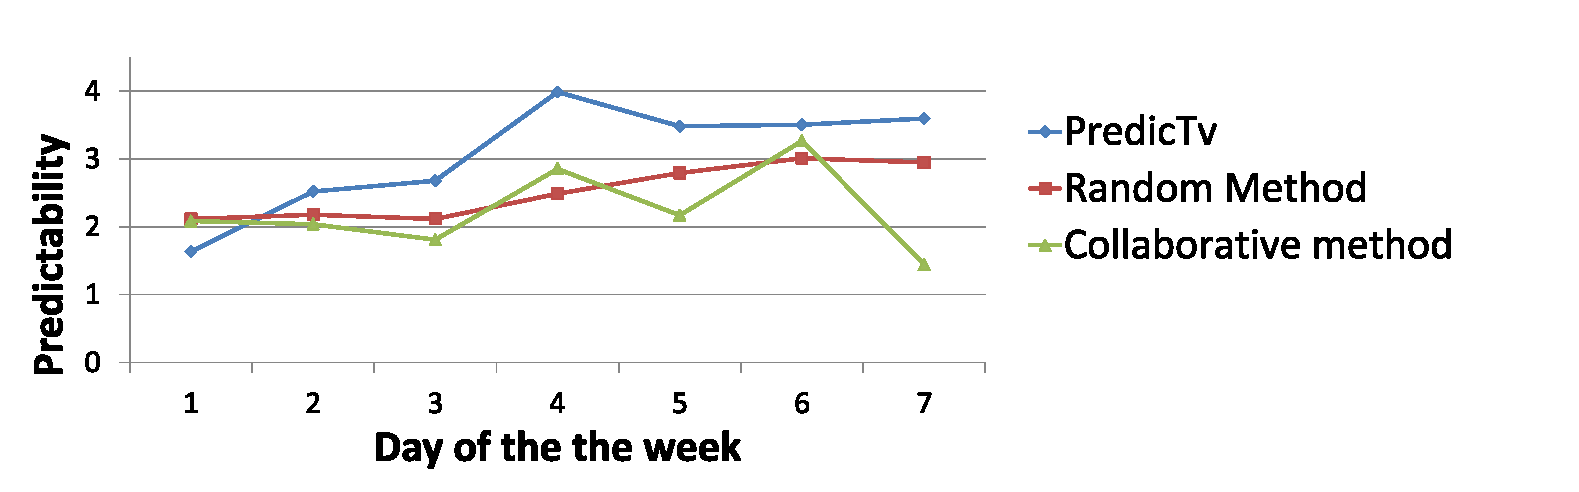
\epsfig{file=precision.eps,width=\columnwidth}
\caption{\label{fig:predict}Predictability curves of the 3 algorithms}
\end{center}
\end{figure}
